\chapter{SP2-CU15 Modificar comentarios a propuesta de Unidad de Aprendizaje}
\begin{UseCase}{SP2-CU15}{ Modificar comentarios a propuesta de Unidad de Aprendizaje }{El usuario podrá modificar los comentarios previamente realizados en la sección de propuesta de Unidad de Aprendizaje que se está revisando.}
		\UCitem{Versión}{\color{Gray}1.0}
		\UCitem{Autor}{\color{Gray}Romero Ponce Mauricio Isaac}
		\UCitem{Supervisa}{\color{Gray}Parra Garcilazo Cinthya Dolores}
		\UCitem{Actor}{Analista}
		\UCitem{Propósito}{Tener oportunidad de modificar el contenido de los comentarios generados previamente en la propuesta de Unidad de Aprendizaje.}
		\UCitem{Entradas}{Las unica entrada para modificar un comentario en una sección de la propuesta de unidad de aprendizaje es:
          \begin{itemize}
          	\item Modificación al comentario anterior.
           % \item fecha en que se genera el nuevo comentario.
            %\item Identificador unico del analista.
          \end{itemize}
        }
		\UCitem{Origen}{Mouse y teclado.}
		\UCitem{Salidas}{
        	\begin{itemize}
        		\hypertarget{CU15-MSG1}{\item MSG1 La operación se ha realizado con éxito.}
            \hypertarget{CU15-MSG3}{\item MSG3 Error: debe agregar un texto al nuevo comentario.}
            \hypertarget{CU15-MSG4}{\item MSG4 Ingrese su comentario en el nuevo campo de la bitácora.}
        	\end{itemize}
        }
		\UCitem{Destino}{Pantalla.}
		\UCitem{Precondiciones}{ Se llamó al caso de uso SP2-CU14}
		\UCitem{Postcondiciones}{
            \begin{itemize}
                \item Se modificará en el sistema el comentario.
                \item Se modificará en el sistema la fecha del comentario.
                \item Se mostrará en la bitácora la modificación del comentario.  
             \end{itemize}  
        }
		\UCitem{Errores}{}
		\UCitem{Estado}{Revisión.}
		\UCitem{Observaciones}{}
\end{UseCase}

%--------------------------- CU TRAYECTORIA PRINCIPAL -------------------------
\begin{UCtrayectoria}{Principal}


    \UCpaso[\UCactor] Presiona el botón \IUbutton{Modificar comentario}. 
    
    \UCpaso Obtiene la fecha actual. 
    
    \UCpaso Actualiza la fecha del comentario al que se presionó el botón \IUbutton{Modificar comentario}.
    
    \UCpaso Muestra el mensaje \MSGref{CU15-MSG4}{Ingrese su comentario en el nuevo campo de la bitácora.}.

    \UCpaso[\UCactor] Cierra el mensaje presionando \IUbutton{Aceptar}.
    
    \UCpaso[\UCactor] Ingresa el nuevo comentario en el input text "comentario".
    
    \UCpaso[\UCactor] Presiona el botón \IUbutton{Aceptar}. \hyperref[SP2-CU15-A]{Trayectoria A}.
    
    \UCpaso Verifica que el campo comentario haya sido contestado. \hyperref[SP2-CU15-B]{Trayectoria B}.

    \UCpaso Guarda la modificación del comentario en la base de datos.

    \UCpaso El sistema muestra el  \MSGref{CU15-MSG1}{La operación se ha realizado con éxito.}.

    \UCpaso[\UCactor] Cierra el mensaje presionando \IUbutton{Aceptar}.


\end{UCtrayectoria}

%------------------------ CU TRAYECTORIA ALTERNARIVA A -------------------------

\label{SP2-CU15-A}
\begin{UCtrayectoriaA}{A}{El usuario presionó \IUbutton{Cancelar}}

  \UCpaso Deja el comentario sin modificaciones.
\end{UCtrayectoriaA}

%------------------------ CU TRAYECTORIA ALTERNARIVA B -------------------------
\label{SP2-CU15-B}
\begin{UCtrayectoriaA}{B}{El sistema detecta que el campo “comentario” se encuentra vacío.} 
    \UCpaso El sistema muestra el mensaje \MSGref{CU15-MSG3}{Error: debe agregar un texto al nuevo comentario.}.
    \UCpaso[\UCactor] Cierra el mensaje presionando \IUbutton{Aceptar}.
    \UCpaso Continúa en el paso 6 de la trayectoria principal del SP2-CU15.
\end{UCtrayectoriaA}

\chapter{Pantallas}
 \begin{figure}
  \centering
    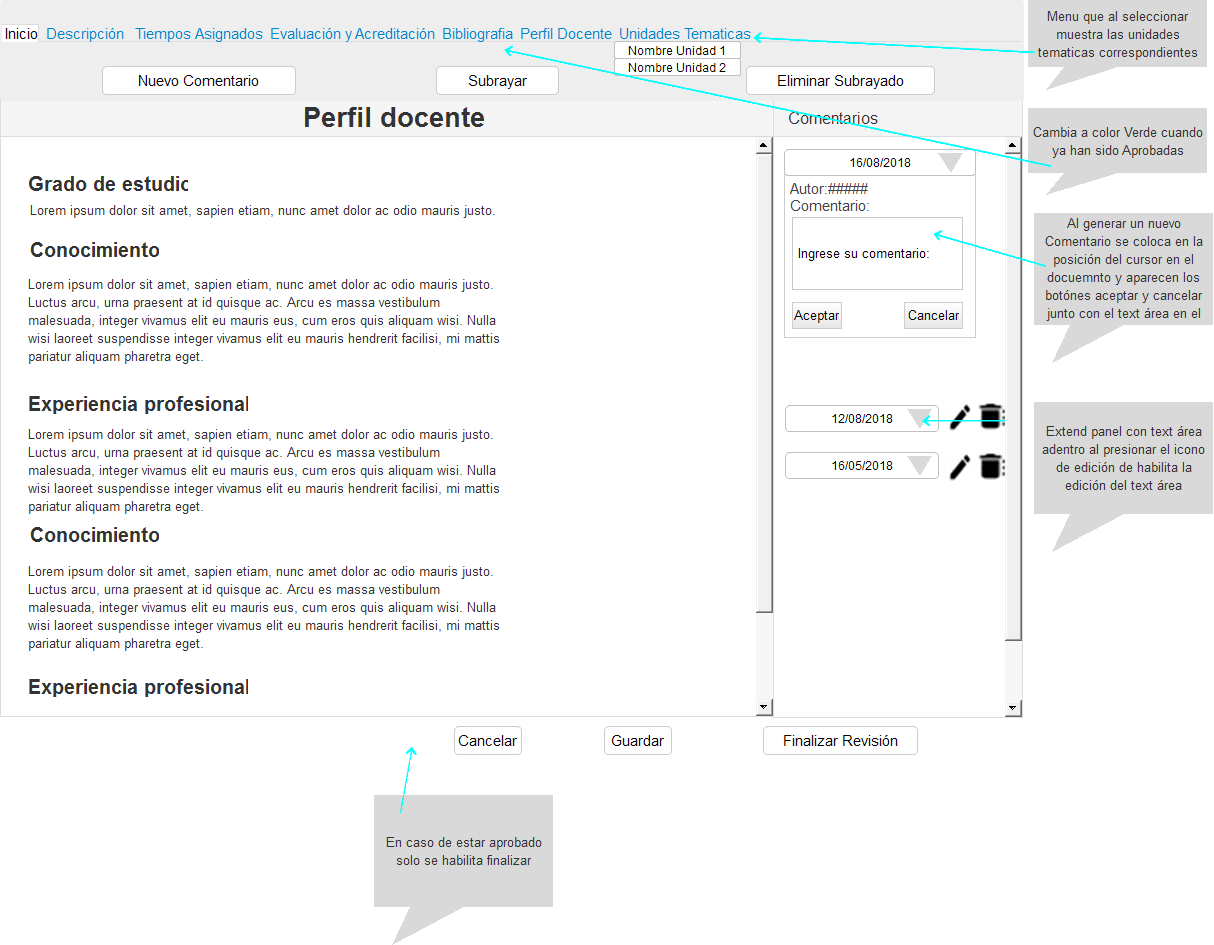
\includegraphics[width=0.7\textwidth]{DCU/SP2/Pantallas/Nuevo_comentario}
  \caption{SP2-IU-Nuevo comentario}
  \label{SP2-IU-Nuevo_comentario}
\end{figure}
